\documentclass{article}
\usepackage[T1]{fontenc}
\usepackage{graphics}
\usepackage{amssymb}
\usepackage{color}

\def\examtitle{}

\def\candidatenumber{39410}
\def\subject{Automata, Logic and Games}
\def\term{Hilary 2005}
\usepackage{oxfordexam}

\def\nat{\mathbb{N}}
\newcommand{\lsem}{[\![}
\newcommand{\rsem}{]\!]}

\def\qedsymbol{$\blacksquare$}
\def\imp{\Longrightarrow}
\def\sem#1{{\lsem #1 \rsem}}
\def\zor{\vee}
\def\zand{\wedge}
\def\znot{\neg}
\def\diamond#1{\langle #1 \rangle}

\begin{document}
 \firstpage


\section*{Question 1}
\begin{itemize}

\item[(a)]

$\alpha \in L$ if and only if after some position $k$, $\alpha$ does
not contain any occurrence of 11 and contains infinitely many
occurrences of 101.

$\alpha \in \sem{(0+1)^*.L'}$ where L' is the language recognizing
the words containing infinitely many 101 but containing no
occurrence of 11.

Consider $\beta \in L'$, after each occurrence of 101 in $\beta$
there must be a 0 (since 11 is not allowed). Moreover, between two
occurrences of 1010, the only two possible sequences of symbols are 0
and 10, this corresponds to the regular expression $(0+10)^*$.

Therefore $L' = \sem{ \left( 1010(0+10)^* \right)^\omega }$ and $L
= \sem{(0+1)^*  \left( 1010(0+10)^* \right)^\omega }$

The following B�chi-automaton recognizes this language:
\begin{center}
  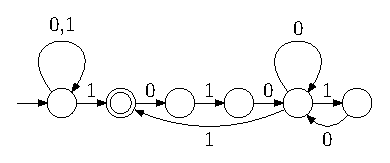
\includegraphics{alg-ex1}
\end{center}


\item[(b)]

Suppose that a deterministic automaton $A = (Q,\{0,1\}, q0, \delta,
F)$ recognizes L. Then $\delta$ is a function and we can extend it
to a function $Q \times \{ 0, 1 \} \rightarrow Q$ returning the
state reached after reading a given sequence of symbols from a given
state.

A must accept $(101)^\omega$, therefore there is a word $w_1 \in
\Sigma^*$ such that $\delta(q_0, w_1) \in F$, where $w_1$ is either
$(101)^{n_1}$, $(101)^{n_1}1$ or $(101)^{n_1}10$ for some $n_1\in
\nat$.


Again, A must accept $w_1.11(101)^\omega$ therefore, there is a
word $w_2 \in \Sigma^*$ such that $\delta(q_0, w_1.11.w_2) \in F$,
where $w_2$ is either $(101)^{n_2}$, $(101)^{n_2}1$ or $(101)^{n_2}10$
for some $n_2\in \nat$.


In this manner, we can create an infinite word $\alpha =
w_1.11.w_2.11.\ldots w_k.11. \ldots$ which is recognized by A since
the corresponding run passes infinitely through states in F. This is
a contradiction, since $\alpha$ contains infinitely many 11 and
therefore cannot belong to L = L(A).

\end{itemize}

\section*{Question 2}

We prove the result by contradiction. Suppose that $\phi(A,B)$,
expressing that A and B have the same number of elements, is
definable in S1S.

We define the S1S formula $\mbox{partition}(A,B,C)$ stating that the
sets $A$, $B$ and $C$ form a partition of $\omega$:
\begin{eqnarray*}
\mbox{partition}(A,B,C) &=& \forall x . (x \in A\ \zor\ x \in B\
\zor\ x
\in C) \\
    && \zand  \forall y .
    \znot \left( (y \in A\ \zand\ y \in B) \zor (y \in A\ \zand\ y \in C) \zor (y \in B\ \zand\ y \in C) \right)
\end{eqnarray*}

We define $\psi(X,Y)$ stating that after an occurrence of an element
in $Y$ there is no occurrence of an element in $X$:
$$ \psi(X,Y) = \forall y. y \in Y \to  ( \forall x . x \geq y \to x \not\in X)$$



We now consider the alphabet $\Sigma = \{ 0, 1 \}^3$. An infinite
word $\alpha$ on $\Sigma$ is defined by three tracks characterized
by the sets $A$, $B$ and $C$:
$$ \forall x \in \omega : \alpha (x) = \left(
\begin{array}{cc}
{ [ x \in A ]} \\
{ [ x \in B ]} \\
{ [ x \in C ]}
\end{array}
\right)$$


We use the following notation:
$$a = \left( \begin{array}{c} 1 \\
0 \\       0
\end{array} \right),
 b = \left( \begin{array}{c}       0 \\       1 \\       0     \end{array}
 \right) \mbox{ and }
 c = \left( \begin{array}{c}       0 \\       0 \\       1     \end{array}
 \right)$$


Then the following formula denotes the language $L = \{ a^n b^n
c^\omega | n \in \nat \}$:

$$\mbox{partition}(A,B,C) \zand \psi(A,B) \zand
\psi(B,C) \zand \psi(A,C) \zand (\exists z . z \in C)$$


Hence $L$ is S1S definable and therefore there is a
non-deterministic B�chi automaton recognizing L (by theorem 3.3 of
the the lecture's notes).

This is a contradiction since $L$ is not regular. Indeed, suppose
that a B�chi-automaton $A$ with $m$ states recognizes $L$. Take $n >
m$, then $a^n b^n c^\omega \in L$. After reading the first $n$
symbols $a$, the automaton has visited twice a particular state.
Suppose this state has been visited after reading $a^i$ and after
reading $a^j$ with $i<j\leq n$. We know that $a^i b^i c^\omega \in
L$. Since $A$ is in the same state after reading $a^i$ and $a^j$, we
also have $a^j b^i c^\omega \in L$ too. This is a contradiction
since $i<j$.

\section*{Question 3}
\begin{itemize}
\item[(a)]
Let us define the following two operators:
$$ A \oplus B \triangleq (A \zor B) \zand \znot (A \zand B)$$
$$ A \leftrightarrow B \triangleq \znot (A \oplus B)$$

Then the following formula $\phi(X,Y,Z)$ expresses that the numbers
$a$,$b$ and $c$ represented respectively by the finite sets $X$,$Y$
and $Z$ are related by the equation $a+b=c$:
\begin{eqnarray*}
\phi(X,Y,Z) &=& \exists R | 0 \not\in R \\
&\zand& \forall b .\ b \in Z \leftrightarrow \left[ (b \in X) \oplus (b \in Y) \oplus (b \in R) \right] \\
&\zand& \forall b .\ \mathbf{s}\ b \in R \leftrightarrow \left(
\left[ (b \in X) \zand (b \in Y) \right] \zor
\left[ (b \in X) \zand (b \in R) \right] \zor
\left[ (b \in Y) \zand (b \in R) \right] \right)
\end{eqnarray*}

The first line states that there is a set $R$ defining the value of the reminder for every step of the binary
addition. $0 \not\in R$ means that there is no reminder for the computation of the digit 0 of $c$.
The second line defines how the semi-addition is done and the third line defines how the reminder is calculated
at every step.

\item[(b)]
For any first-order formula $\psi$ over the structure $(\omega,+)$,
we can construct an equivalent S1S formula $F(\psi)$ as follow:

Let $x$, $y$ and $z$ be first order variables, we define corresponding
second order $\mu$-calculus variables $X$, $Y$ and $Z$. $F$ is defined recursively as follow:
\begin{eqnarray*}
F ( \psi_1 \zand \psi_2 ) &=& F( \psi_1 ) \zand F(\psi_2) \\
F ( \psi_1 \zor \psi_2 ) &=& F( \psi_1 ) \zor F(\psi_2) \\
F ( \znot \psi ) &=& \znot F( \psi )  \\
F ( \forall x . \psi ) &=& \forall X . F( \psi ) \\
F ( \exists x . \psi ) &=& \exists X . F( \psi ) \\
F ( x + y = z ) &=& \phi (X,Y,Z) \\
F ( x ) &=& X
\end{eqnarray*}
Moreover for any constant $n \in \omega$ we define $F( n )$ as the
set of numbers corresponding to the position of 1's in the binary representation of $n$:
$$F ( n ) = \{ k \in \nat | \mbox{ the $k^{th}$ binary digit in the binary representation of $n$ is a 1} \} $$


A Presburger arithmetic formula $\phi(x_1,\ldots,x_n)$ can be transformed into the S1S formula
$F(\phi(x_1,\ldots,x_n)) = \psi(X_1,\ldots X_n)$. From this S1S formula, we can construct the B�chi automaton
$A_\psi$ defines in slide 3-17 of the lecture's note. The language recognized by this automaton is not empty if and only
if the formula $\psi$ is satisfiable. Hence, since non-emptyness is decidable for B�chi automata (theorem 1.6), Presburger arithmetic
is decidable.

\item[(c)]
What we proved is that when we encode numbers into sets, we can decide whether the second-order variable
$X$, $Y$ and $Z$ encode numbers satisfying the relation $x + y = z$.

But if $x$, $y$ and $z$ are first-order variables then the natural number addition $x + y = z$ on these
first-order variables is not definable in S1S.

\end{itemize}

\section*{Question 4}
See answer on the attached sheets.
\clearpage\ \clearpage\ \clearpage\ \clearpage\ \clearpage\

\section*{Question 5}

\begin{itemize}
\item[(a)]

\def\musem#1{\| #1 \|_\emptyset^T}

We define the following two functions:
\begin{eqnarray*}
\Phi(X,Z) &=& [a] (( Z \zor \diamond{b} t ) \zand X ) \\
\phi(X) &=& \mu Z . \Phi(X,Z)
\end{eqnarray*}

Let us first do some preliminary computations:
\begin{itemize}
\item We have:
\begin{eqnarray*}
    \musem{\mu^0 Z . \Phi(S,Z) } &=& \emptyset \\
    \musem{\mu^1 Z . \Phi(S,Z) } &=& \musem{ [a] ( \underbrace{\diamond{b} t}_{\{1\}}) } = \{2 \} \\
    \musem{\mu^2 Z . \Phi(S,Z) } &=& \musem{[a] ( \underbrace{\{ 2\} \zor \{ 1\}}_{\{1,2\}}) } = \{1,2 \} \\
    \musem{\mu^3 Z . \Phi(S,Z) } &=& \musem{[a] ( \{ 1,2\} \zor \{1\}) } = \{1,2 \}
\end{eqnarray*}
therefore:
\begin{eqnarray}
    \musem{\phi(S)} = \musem{\mu Z . \Phi(S,Z) } &=& \{1,2 \}  \label{eq1}
\end{eqnarray}

\item moreover:
\begin{eqnarray*}
    \musem{\mu^0 Z . \Phi(\{1,2\},Z) } &=& \emptyset \\
    \musem{\mu^1 Z . \Phi(\{1,2\},Z) } &=&    \musem{ [a] ( \{1\} \zand \{1,2\} ) }    = \musem{ [a] ( \{1\} ) } = \{ 2\} \\
    \musem{\mu^2 Z . \Phi(\{1,2\},Z) } &=&    \musem{[a] ( ( \{2\} \zor \{1\}) \zand \{1,2\} ) } =    \musem{[a] ( \{1,2\} ) } =    \{1,2\} \\
    \musem{\mu^3 Z . \Phi(\{1,2\},Z) } &=&  \musem{[a] ( ( \{1,2\} \zor \{1\}) \zand \{1,2\} ) } = \musem{[a] ( \{1,2\} ) }  = \{1,2 \}
\end{eqnarray*}
therefore:
\begin{eqnarray}
    \musem{\phi(\{1,2\}) } = \musem{\mu Z . \Phi(\{1,2\},Z) } = \{1,2 \}  \label{eq2}
\end{eqnarray}

\end{itemize}


We can compute the fixpoint approximants for $\musem{\nu X . \phi(X)}$:
\begin{eqnarray*}
    \musem{\nu^0 X . \phi(X)} &=& S\\
    \musem{\nu^1 X . \phi(X)} &=& \musem{ \phi(S) } = \{1,2\} \quad \mbox{ (equation \ref{eq1})} \\
    \musem{\nu^2 X . \phi(X)} &=& \musem{ \phi(\{1,2\}) } = \{1,2\} \quad \mbox{ (equation \ref{eq2})}
\end{eqnarray*}

Hence $\musem{\nu X . \phi(X)} = \{ 1,2\}$.

\item[(b)]
The following graph describes the game $\mathcal{G}_\emptyset^T\left( 2, \mu Z. \nu X. ([a](Z \zor \diamond{b} t)
\zand [b] X) \right)$:
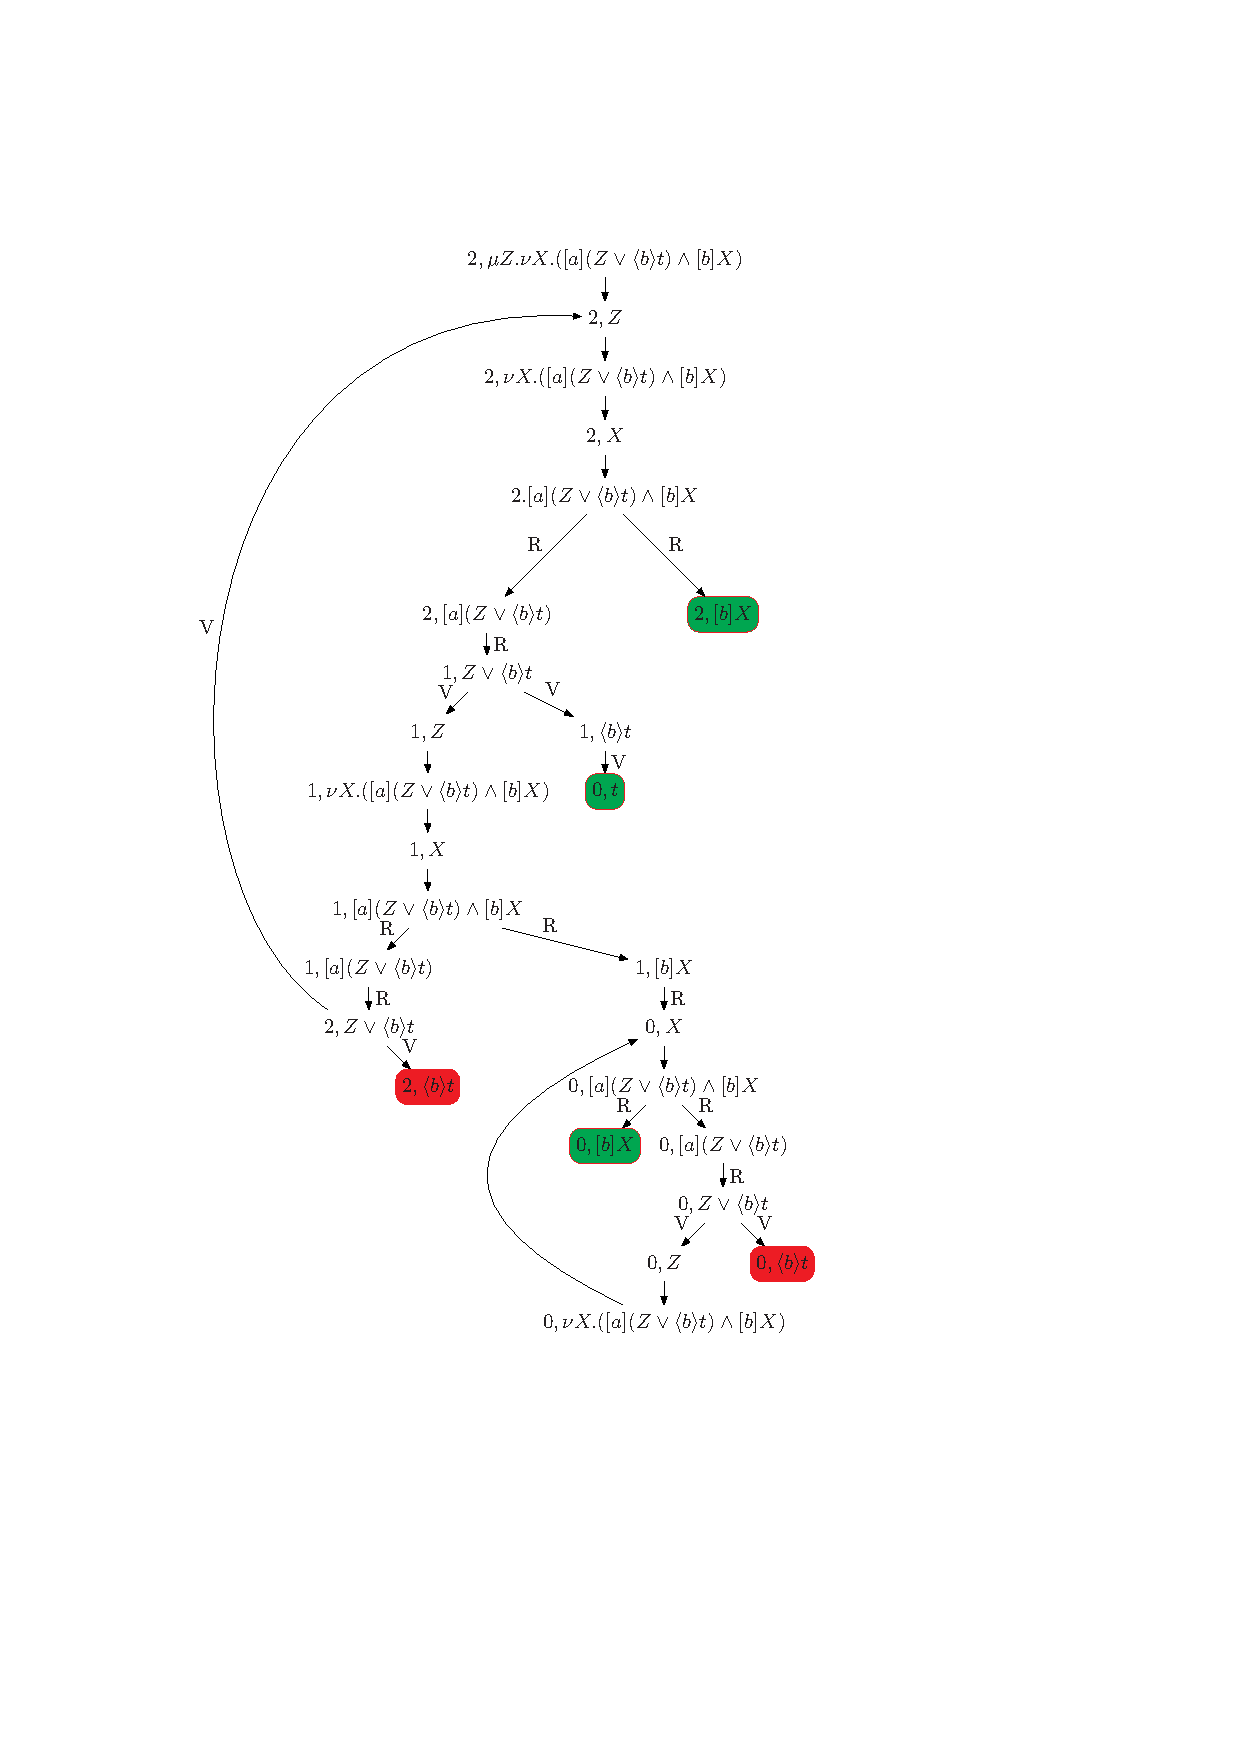
\includegraphics{alg-ex5}

The \textcolor{green}{green} position correspond to the verifier's winning positions, the \textcolor{red}{red} positions correspond to the refuter's
winning position.

We recall theorem 5.2 from the notes:
\newtheorem{theorem}{Theorem}
\begin{theorem}
\begin{enumerate}
\item $s \models_V^T \phi$ iff player V has as history-free winning strategy for $\mathcal{G}_V^T(s,\phi)$
\item $s \not\models_V^T \phi$ iff player R has as history-free winning strategy for $\mathcal{G}_V^T(s,\phi)$
\end{enumerate}
\end{theorem}


V has a history-free winning strategy for $\mathcal{G}_\emptyset^T\left( 2, \mu Z. \nu X. ([a](Z \zor \diamond{b} t)
\zand [b] X) \right)$ consisting in choosing the position ``$1,\diamond{b} t$'' when the game is at position
``$1,Z\zor \diamond{b}t$''. Hence $ 2 \models \mu Z. \nu X. ([a](Z \zor \diamond{b} t)
\zand [b] X)$.

\end{itemize}

\section*{Question 6}
\begin{itemize}
  \item[(a)]
\begin{eqnarray*}
  \alpha \models \mathbf{X} \phi \to \mathbf{X} \psi &\iff& (\alpha \models \mathbf{X} \phi) \imp (\alpha \models \mathbf{X} \psi) \\
            &\iff& (\alpha^1 \models \phi) \imp (\alpha^1 \models \psi) \\
            &\iff& \alpha^1 \models (\phi \to \psi) \\
            &\iff& \alpha \models \mathbf{X} (\phi \to \psi)
\end{eqnarray*}

  \item[(b)]
\begin{eqnarray}
\alpha \models \phi\ \mathbf{R}\ \psi &\iff& \forall k \geq 0 . (\alpha^k \models \psi\ \zor\ \exists i : 0 \leq i < k . \alpha^i \models \phi ) \nonumber \\
    &\iff& \qquad \left[ \alpha \models \psi\ \zor\ \overbrace{\exists i : 0 \leq i < 0 . \alpha^i \models \phi}^{false} \right] \qquad\qquad\qquad\qquad (k=0) \nonumber \\
        && \zand \underbrace{\forall k > 0 . (\alpha^k \models \psi\ \zor\ \exists i : 0 \leq i < k . \alpha^i \models \phi )}_{A} \nonumber \\
    &\iff& \alpha \models \psi
        \zand \left[ (A \zand \alpha \models \psi) \zor (A \zand \alpha \not\models \psi) \right] \label{eq3}
\end{eqnarray}

\begin{itemize}
\item Since
$$ \alpha \models \phi \qquad \imp \qquad \left[ \forall k>0 . \exists i:0\leq i < k .\alpha^i \models \phi \right] \equiv A$$
we have $ (A \zand \alpha \models \psi) \quad \equiv \quad \alpha \models \phi$.

\item Moreover,
\begin{eqnarray*}
A \zand \alpha \not\models \phi &\imp& \forall k>0 . (\alpha^k \models \psi  \zor \exists i:0<i<k.\alpha^i \models \phi) \\
&\stackrel{k\leftarrow k-1}{\iff}& \forall k\geq 0 . (\alpha^{k+1} \models \psi  \zor \exists i:0<i<k+1.\alpha^i \models \phi) \\
&\stackrel{i\leftarrow i-1}{\iff}& \forall k\geq 0 . (\alpha^{k+1} \models \psi  \zor \exists i:0\leq i<k.\alpha^{i+1} \models \phi) \\
&\iff& \forall k\geq 0 . ( (\alpha^1)^k \models \psi  \zor \exists i:0\leq i<k.(\alpha^1)^i \models \phi) \\
&\stackrel{R \mbox{ def.}}{\iff}& \alpha^1 \models \phi\ \mathbf{R}\ \psi \\
&\imp& \alpha \models  \mathbf{X} (\phi\ \mathbf{R}\ \psi)
\end{eqnarray*}
\end{itemize}

By plugging these two results into equation \ref{eq3} we obtain the desired result:
$$
\alpha \models \phi\ \mathbf{R}\ \psi \imp
 \alpha \models \psi
        \zand \left[ \alpha \models \phi \zor  \alpha \models  \mathbf{X} (\phi\ \mathbf{R}\ \psi)  \right]
$$

  \item[(c)]
We first prove the identity $\textrm{f}\ \mathbf{R}\ \phi = \mathbf{G} \phi$:
\begin{eqnarray*}
\alpha \models \textrm{f}\ \mathbf{R}\ \phi &\iff& \forall k \geq 0 . \alpha^k \models \phi \ \zor\ \exists i:0\leq i<k : \alpha^i \models \textrm{f} \\
&\iff& \forall k \geq 0 . \alpha^k \models \phi \\
&\iff& \alpha \models \mathbf{G} \phi
\end{eqnarray*}

Hence:
\begin{eqnarray*}
\textrm{f}\ \mathbf{R}\ (\phi \zand \mathbf{X} \phi) \to ( \phi \to \textrm{f}\ \mathbf{R} \phi )
&\equiv&
\mathbf{G} (\phi \zand \mathbf{X} \phi) \to (\phi \to \mathbf{G} \phi) \\
&\equiv&
\mathbf{G} \phi \to (\phi \to \mathbf{G} \phi) \\
&\equiv&
(\mathbf{G} \phi  \zand \phi ) \to (\mathbf{G} \phi) \\
&\equiv&
\mathbf{G} \phi  \to (\mathbf{G} \phi) \\
&\equiv&
\mathbf{true}
\end{eqnarray*}


\item[(d)] \textbf{Claim}: $\phi\ \mathbf{R}\ \psi \equiv \mathbf{G} (\znot \phi \zand \psi)\ \zor\ (\znot\phi \zand\psi) \mathbf{U} (\phi \zand\psi) $

\textbf{Proof}:
We first note that $\phi\ \mathbf{R}\ \psi \equiv \left[ (\phi\ \mathbf{R}\ \psi) \zand \mathbf{G} \znot \phi \right]\ \zor\
    \left[ (\phi\ \mathbf{R}\ \psi) \zand \mathbf{F} \phi \right]$

\begin{itemize}
  \item We have $ (\phi\ \mathbf{R}\ \psi) \zand \mathbf{G} \znot \phi\ \equiv\ \mathbf{G} (\znot \phi \zand \psi)$,
  indeed:
  \begin{eqnarray*}
    \alpha \models (\phi\ \mathbf{R}\ \psi) \zand \mathbf{G} \znot \phi  &\iff&
\left( \forall k \geq 0 . \alpha^k \models \psi \zor \exists i : 0 \leq i < k . \alpha^i \models \phi \right)
\zand ( \forall l \geq 0 : \alpha^l \models \znot \phi) \\
&\iff& \forall k \geq 0 : (\alpha^k \models \psi \zand \forall l \geq 0 : \alpha^l \models \znot \phi) \\
&&    \zor \underbrace{\left[ (\exists  i : 0 \leq i <k.\alpha^i \models \phi) \zand (\forall l \geq 0 : \alpha^l \models \znot \phi) \right]}_{false} \\
&\iff& \forall k \geq 0 : \alpha^k \models \psi \zand \forall l \geq 0 : \alpha^l \models \znot \phi \\
&\iff& \alpha \models \mathbf{G} (\znot \phi \zand \psi)
  \end{eqnarray*}

  \item moreover $ (\phi\ \mathbf{R}\ \psi) \zand \mathbf{F} \phi\ \equiv\ (\znot\phi \zand\psi) \mathbf{U} (\phi \zand\psi)$, indeed:
  \begin{eqnarray*}
    \alpha \models (\phi\ \mathbf{R}\ \psi) \zand \mathbf{F} \phi &\iff&
        (\forall k \geq 0 :\alpha^k \models \psi \zor \exists i :0\leq i<k:\alpha^i \models \phi) \\
        &&\zand
        (\exists i_0 . \alpha^{i_0} \models \phi \zand \forall j < i_0 : \alpha^j \models \znot \phi) \\
    &\iff& \exists i_0 . \alpha^{i_0} \models \phi \zand (\forall j < i_0 : \alpha^j \models \znot \phi) \\
    && \zand (\forall k \geq 0 :\alpha^k \models \psi \zor \exists i :0\leq i<k:\alpha^i \models \phi) \\
    &\iff& \exists i_0 . \alpha^{i_0} \models \phi \zand (\forall j < i_0 : \alpha^j \models \znot \phi) \\
    && \zand (\forall k < i_0 :\alpha^k \models \psi \zor \exists i :0\leq i<k:\alpha^i \models \phi) \\
    && \zand (\alpha^{i_0} \models \psi \zor \exists i :0\leq i<i_0:\alpha^i \models \phi) \\
    && \zand (\forall k > i_0 :\alpha^k \models \psi \zor \exists i :0\leq i<k:\alpha^i \models \phi) \\
    &\iff& \exists i_0 . \alpha^{i_0} \models \phi \zand (\forall j < i_0 : \alpha^j \models \znot \phi) \\
    && \zand \forall k < i_0 :\alpha^k \models \psi \\
    && \zand \alpha^{i_0} \models \psi \\
    && \zand (\forall k > i_0 :\alpha^k \models \psi \zor \exists i :0\leq i<k:\alpha^i \models \phi) \\
    &\iff& \exists i_0 . \alpha^{i_0} \models \phi \zand (\forall j < i_0 : \alpha^j \models \znot \phi) \\
    && \zand \forall k < i_0 :\alpha^k \models \psi \\
    && \zand \alpha^{i_0} \models \psi \\
    && \zand \forall k > i_0 . \\
    && \qquad [ \left( \alpha^{i_0} \models \phi \zand \alpha^k \models \psi \right)
    \zor
    \underbrace{\left( \alpha^{i_0} \models \phi \zand  \exists i :0\leq i<k:\alpha^i \models \phi \right)}_{\alpha^{i_0} \models \phi} ]\\
    &\iff& \exists i_0 . \alpha^{i_0} \models \phi \zand (\forall j < i_0 : \alpha^j \models \znot \phi) \\
    && \zand \quad \forall k < i_0 :\alpha^k \models \psi \\
    && \zand \quad \alpha^{i_0} \models \psi \\
    && \zand \quad
     \underbrace{\left( \alpha^{i_0} \models \phi \zand \forall k > i_0. \alpha^k \models \psi \right)
    \zor \alpha^{i_0} \models \phi}_{\alpha^{i_0} \models \phi} \\
    &\iff& \exists i_0 . (\forall j < i_0 : \alpha^j \models \znot \phi)\zand (\forall k < i_0 :\alpha^k \models \psi) \\
    && \zand \quad \alpha^{i_0} \models (\psi \zand \phi) \\
    &\iff& \exists i_0 . \forall j < i_0 : \alpha^j \models \znot \phi \zand \psi\\
    && \zand \quad \alpha^{i_0} \models (\psi \zand \phi) \\
    &\iff& \alpha \models (\znot\phi \zand\psi) \mathbf{U} (\phi \zand\psi)
  \end{eqnarray*}
\qedsymbol

\end{itemize}

\end{itemize}

\section*{Question 7}


Suppose that a formula $\phi$ has a model. Then there is a
transition system $T = \langle S, \to, \rho \rangle$ and a state $r
\in S$ such that $r \models_T \phi$.

\begin{itemize}
\item The model $T$ can be unwound into a tree rooted at $r$: the graph of the
transition system is browsed from $r$ in a breadth-first search
manner, every time we reach an edge $s \to t$ where $t$ has already
been visited, we replace the edge $s \to t$ by an edge pointing to a
newly created tree obtained by unwinding the LTS at state $t$. This
process clearly removes all the cycles in the graph, hence the
resulting model is a tree but possibly with an infinite depth.

It is also obvious that $s$ satisfies $\phi$ in this new model: for
a given state, the possible outcomes are the same in the two models.

\item We need to prove that the resulting tree has a bounded width.

We achieve this by assuming with no proof that the small model
property is true for the modal $\mu$-calculus.

The small model property states that if a formula has a model then
it has a model with finite number of states.

By unwinding the finite model, we obtain a tree model with possibly
infinite depth (if there are loops in the finite model) but with a
bounded width. Indeed, the unwinding process preserves the number of
outgoing edges for a node: there may be infinitely many copies of a
node but for all these copies, the number of outgoing edges is the
same as the original node. The number of outgoing edges for a node
is clearly bounded by $|S| . | \mathcal{L}|$ where $\mathcal{L}$ is
the labeling set.
\end{itemize}

\end{document}
